\documentclass{article}
\usepackage{amsmath}
\usepackage{mathtools}
\usepackage{framed} %for important notes that need to be framed
\usepackage{tikz}
\usepackage{multicol} %for multi-column bullet points
\usepackage{float} %for placing figures at the exact place as in the code
\usepackage{lscape} %for inserting landscape pages

\usepackage[a4paper, total={7in, 10in}]{geometry} %for formatting the sheet size

\usepackage{graphicx}
\graphicspath{ {./visualizations/} } %for inserting figures

\usepackage{hyperref} %for hyperlinks
\hypersetup{
    colorlinks = true,
    linkcolor = blue,
    filecolor = magenta,
    urlcolor = cyan,
}


%the comments are from Udacity's project proposal template: https://github.com/udacity/machine-learning/blob/master/projects/capstone/capstone_proposal_template.md

\title{Udacity Machine Learning Nanodegree - Capstone Project}
%(approx. 10-15 pages)
\author{Ruslan Kozhuharov}

\begin{document}
\pagenumbering{gobble}
\maketitle
\tableofcontents
\newpage
\pagenumbering{arabic}
\setlength{\parskip}{1em}

\section{Definition}
%(approx. 1-2 pages)
\subsection{Project Overview}
%In this section, look to provide a high-level overview of the project in layman’s terms. Questions to ask yourself when writing this section:
%Has an overview of the project been provided, such as the problem domain, project origin, and related datasets or input data?
%Has enough background information been given so that an uninformed reader would understand the problem domain and following problem statement?
The Kiva organization is a charitable entity that funds underprivileged people around the world through small loans. Such loans are funded on Kiva’s online platform by one or several donors. The loan amount is then disbursed by Kiva associates to financially excluded individuals. Kiva itself does not collect rent on those loans, but Kiva associates could in order to cover their operating costs. Once a loan is repaid, the individual donors could choose another cause and continue their charitable activity. This helps poor communities by:
\begin{itemize}
  \item Fostering economic activity
  \item Providing access to funds for financially excluded individuals
  \item Encouraging entrepreneurial initiative on the part of the borrower
\end{itemize}
In order to improve their reach, however, Kiva needs a good assessment of the poverty levels in their areas of operation. To do that, Kiva has requested in a \href{https://www.kaggle.com/kiva/data-science-for-good-kiva-crowdfunding}{Kaggle challenge} that a poverty score is created based on other data and that score is combined with a data set for Kiva’s loans from the last 2 years.

The prior research in this area consists of two main bodies: the \href{https://en.wikipedia.org/wiki/Human_Poverty_Index}{Human Poverty Index}, developed in 1997 and the \href{https://en.wikipedia.org/wiki/Multidimensional_Poverty_Index}{Multidimensional Poverty Index}, introduced in 2010. The Human Poverty Index (HPI) focuses on the following metrics for defeloping countries:

\begin{itemize}
  \item Mortality
  \item Illiteracy
  \item Living conditions (access to water and access to nutrition)
\end{itemize}

For the so called 'high income OECD countries', the HPI uses the following metrics:

\begin{itemize}
  \item Mortality
  \item Illiteracy
  \item Income
  \item Unemployment
\end{itemize}

The HPI is statistically-derived result that uses the formula:

\begin{equation}
  HPI = \Bigg[ \frac{\sum_{i = 1}^{n} P_i^\alpha}{n} \Bigg]^{\frac{1}{\alpha}}
\end{equation}

That is, the HPI is not predictive, but descriptive. In 2010, the HPI was replaced by the Multidimensional Poverty Index (MPI). As with the HPI, the MPI is a descriptive index. The MPI is based on more aspects of poverty, namely:

\begin{itemize}
  \item Child mortality
  \item Nutrition
  \item Years of education
  \item School attendance
  \item Energy and electricity
  \item Water
  \item Sanitation
  \item Accomodation
  \item Assets
\end{itemize}

The indicators above have different weights in the index and their sumproduct is weighted by the so-defined poverty's intensity.

We will attempt to develop a predictive model that uses various factors mentioned above as predictors of lack of income. In this respect our model is more singular than the HPI and MPI, but on the other hand could use the indicators present in both indices as predictors.

\hypertarget{prob_statement}{\subsection{Problem Statement}}
%In this section, you will want to clearly define the problem that you are trying to solve, including the strategy (outline of tasks) you will use to achieve the desired solution. You should also thoroughly discuss what the intended solution will be for this problem. Questions to ask yourself when writing this section:
%Is the problem statement clearly defined? Will the reader understand what you are expecting to solve?
%Have you thoroughly discussed how you will attempt to solve the problem?
%Is an anticipated solution clearly defined? Will the reader understand what results you are looking for?
Based on the definition of the Kiva challenge laid out in the Project Overview, the problems we are going to solve are the following:
\begin{enumerate}
  \item Defining the mathematical expression of ‘poverty’
  \item Selecting the necessary regional data sets
  \item Transforming the data set from step 2 to a form usable for modeling
  \item Building the poverty prediction model
  \item Joining the predicted poverty to all records of the Kiva loans data set
\end{enumerate}
\subsubsection{Defining Poverty}
As mentioned above, ‘poverty’ is a subjective notion that we need to convert to a mathematical measure. In defining that measure we need to take into account the following factors:
\begin{itemize}
  \item The measure should be applicable on country as well as on global level.
  \item The measure should be on a scale between 0 to 1 so that it represents a percentage of poverty. This will allow Kiva to report on poverty-affected areas with regards to the measure’s maximum.
  \item The measure should be scalable if corresponding data from more countries is added.
\end{itemize}
With regards to these points, we will define the poverty score as: 1 - predicted normalized total household income. That is, poverty score of 0.8 corresponds to predicted normalized total household income of 0.2. Thus our prediction will always be on scale from 0 to 1, will be applicable to country and global levels and will be scalable as more country profiles are added (the normalized household income will always be from 0 to 1).
\subsubsection{Selecting Data Sets}
There are two main problems that need to be resolved when selecting data sets useful for the modeling task:
\begin{itemize}
  \item Data with the widest possible coverage (World Bank, UN statistics, CIA World Factbook) is averaged out for each country and does not present a nuanced enough picture of the poverty levels. That is, in countries with high GINI coefficient, the average income levels do not provide a sufficient information about areas with a significant deviation from the average (poverty affected areas).
  \item Local country data is presented in different formats. Every country measures different macroeconomic indicators (and sometimes measures the same indicators in different ways). This makes local data, that could eventually be joined together on global level, unreliable. Example: some countries may consider 'unemployment' as the number of working age individuals with no regular employment contract as unemployed. Other countries may consider 'unemployment' as individuals who do not have a regular employment contract AND are looking for employment (i.e. individuals who are not actively looking for jobs are not counted).
\end{itemize}

To address these issues, we will select the country where Kiva grants the highest number of loans. We will focus exclusively on that country and find a detailed dataset, preferably containing raw data. We will then build an adequate model for the selected country and reduce the number of variables to a few, easily obtainable for other countries. This will make our model, although localized, scalable.

The country receiving the most Kiva loans at this point is the Philippines. Therefore, we will use data from the \href{https://www.kaggle.com/grosvenpaul/family-income-and-expenditure}{Philippines Family Income and Expenditure triennial survey (FIES)}. The data contains information about families’ incomes, expenses, and living conditions (with detailed information about accommodation types, running water, electricity, communications devices, family size, education, etc.). The data set is published on Kaggle and is produced by the Philippines Statistics Authority (PSA).

This data set will be used to derive a model that can predict poverty out of the available features. The poverty score will then be grouped by region and household head gender. We will also derive the administrative regions from the Kiva data set and join the calculated poverty score by region and gender of the borrower.

\subsubsection{Transforming The Data}
Since the data set we will utilize will contain raw data, we will need to transform it to numerical or one hot encoded features. We will perform this work separately in a data transformation phase.
\subsubsection{Building The Poverty Prediction Model}
Once we have transformed the FIES data, we will need to find eventual correlations, remove irrelevant fields and prepare for modeling. We will then proceed and try the effectiveness of several out of the box models (we will refer to them as ‘candidate models’) against three dummy predictors.

The dummy predictors will always predict poverty scores of 0, 0.5 and 1, respectively. We will then compare the performance of the candidate models against the dummy predictors based on the evaluation metrics defined in the next chapter. Finally, we will select the best performing model and improve on it.

The improvement will consist of selecting the features with highest predictive potential and discarding the rest. This will allow Kiva to easily integrate the model in their operation (by simply adding the 3-5 new questions to their loan application form).
\subsubsection{Joining The Predicted Poverty To Existing Kiva Data}
In this phase, we will find an appropriate way to join the results of the poverty prediction model to the existing Kiva loans data set. We will join the poverty scores by borrower gender and region.
\subsection{Metrics}
%In this section, you will need to clearly define the metrics or calculations you will use to measure performance of a model or result in your project. These calculations and metrics should be justified based on the characteristics of the problem and problem domain. Questions to ask yourself when writing this section:
%Are the metrics you’ve chosen to measure the performance of your models clearly discussed and defined?
%Have you provided reasonable justification for the metrics chosen based on the problem and solution?
We will utilize the following evaluation metrics for the household income prediction:
\begin{itemize}
  \item Mean squared error:
    \begin{equation}
      MSE(y, \hat{y}) = \frac{1}{n_{samples}}\sum_{i=0}^{n_{samples} - 1}(y_i - \hat{y}_i)^2
    \end{equation}
  \item R2 score:
    \begin{equation}
      R^2(y, \hat{y}) = 1 - \frac{\sum_{i=0}^{n_{samples} - 1}(y_i - \hat{y}_i)^2}{\sum_{i=0}^{n_{samples} - 1}(y_i - \bar{y}_i)^2}
    \end{equation}
  \item Mean squared logarithmic error:
    \begin{equation}
      MSE(y, \hat{y}) = \frac{1}{n_{samples}}\sum_{i=0}^{n_{samples} - 1}(log_e(1 + y_i) - log_e(1 + \hat{y}_i))^2
    \end{equation}
  \item Explained variance score:
    \begin{equation}
      EV(y, \hat{y}) = 1 - \frac{Var\{y - \hat{y}\}}{Var\{y\}}
    \end{equation}
\end{itemize}

As evident by our choice, we want to focus on two metrics for the errors in our model and two metrics to help us understand the model's robustness and potential future performance. The mean squared error and the mean squared logarithmic error will allow us to assess the deviation of our model's prediction from the target variable.

We will also utilize the R2 score (the coefficient of determinations) - a mtric that represents the future performance of the model (how accurately new samples are expected to be predicted by the same model). Using this metric will allow us to build a robust model that could generalize well on new data.

The explained variance score will allow us to assess how our model accounts for the deviation from the mean within our sample. This is important for us as we are trying to predict a spectrum of poverty. Or model is expected to account for the nuances of our target variable in the various regions where data is available. Therefore, we have to take the explained variance score into account as we refine our model.

\section{Analysis}
%(approx. 2-4 pages)
\subsection{Data Exploration}
%In this section, you will be expected to analyze the data you are using for the problem. This data can either be in the form of a dataset (or datasets), input data (or input files), or even an environment. The type of data should be thoroughly described and, if possible, have basic statistics and information presented (such as discussion of input features or defining characteristics about the input or environment). Any abnormalities or interesting qualities about the data that may need to be addressed have been identified (such as features that need to be transformed or the possibility of outliers). Questions to ask yourself when writing this section:
%If a dataset is present for this problem, have you thoroughly discussed certain features about the dataset? Has a data sample been provided to the reader?
%If a dataset is present for this problem, are statistics about the dataset calculated and reported? Have any relevant results from this calculation been discussed?
%If a dataset is not present for this problem, has discussion been made about the input space or input data for your problem?
%Are there any abnormalities or characteristics about the input space or dataset that need to be addressed? (categorical variables, missing values, outliers, etc.)
We are using two main data sets: the Kiva loans dataset and the Philippines Family Income and Expenditure Survey (FIES). Both of the datasets are not immediately suitable for the tasks laid out in the \hyperlink{prob_statement}{Problem Statement}. This means that we will have to transform the data in certain ways. We will now look at each data set and its corresponding data transformation.
\subsubsection{Kiva Loans Data Set}
The Kiva loans data set contains 671205 records for loans granted by Kiva in the last 2 years. For the purpose of this project we will use the following columns:
\begin{itemize}
  \item Id: The unique identifier for each loan record. It has a numeric value.
  \item Country: The name of the country where the loan was granted in camel case. We will use this column to select all records from the Philippines.
  \item Region: Unstructured representation of an administrative entity that is below the level of a country. The entity could be a city, city and a province name separated by comma, village name, other geographic entities or no value. We will use this column to derive the actual administrative region in the Philippines where the loan was granted. The derived administrative region will be further used to join the poverty score by region.
  \item Borrower\_gernders: The unique categories in this column are ‘male’ and ‘female’. However, the column’s values could be any combination of those two that is as long as the number of borrowers (e.g. ‘female’, ‘female’, ‘male’ for 3 borrowers of the same loan record). We use this column to derive a borrower gender female one hot encoded column. The new column will be subsequently used to join the poverty score by gender.
\end{itemize}
Here is a sample of the contents of the above-mentioned columns for 5 records:

\begin{center}
\begin{tabular}{ |l|l|l|l| }
  \hline
  id & country & region & borrower\_genders \\
  \hline
  1209550 & Philippines & Dipolog -Zamboanga del Norte & female \\
  888025 & Nicaragua & Masaya & female, female, female \\
  1171969 & Philippines & Roxas Palawan & female \\
  867403 & El Salvador & NaN & male \\
  742400 & Nigeria & Kaduna & female \\
  \hline
\end{tabular}
\end{center}

As we can see from this short example, the ‘region’ column could contain a ‘<city> <province>’ tuple (for loan id 1209550, where the city is Dipolog and the province is Zamboanga del Norte), only city (Masays for loan id 888025), municipality name (Roxas Palawan for loan id 1171969) or no valid value (‘NaN’ for loan id 867403). We will need to transform this column to a standard value using matching tables and other heuristics.

For the records from the Philippines, the unique values for the ‘borrower\_genders’ column are only: ‘female’, ‘male’ and NaN. That’s why will also transform the ‘borrower\_genders’ column by mapping the ‘female’ category to 1 and the ‘male’ category to 0. There are only 80 records with missing values (NaN), so we could do away with them.

Let us now take a look into some key characteristic distributions. The borrower gender distribution seems to be skewed strongly in favor of female borrowers:

\begin{figure}[H]
\caption{Number of Loans Per Region}
\centering
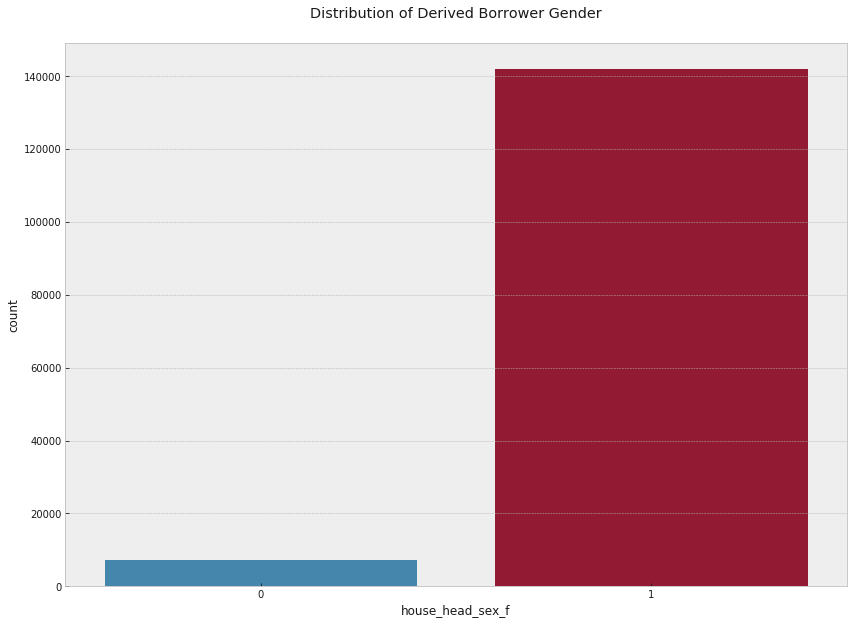
\includegraphics[width = 0.7 \textwidth]{borrower_gender_distribution}
\end{figure}



\subsubsection{Philippines Family Income and Expenditure Survey}
The Philippines Family Income and Expenditure Survey (FIES) contains 41544 records of household incomes, expenditure, living conditions and other affluence indicators. The data set contains 59 columns representing information in the following categories:

\begin{itemize}
  \item Demographics
    \begin{multicols}{2}
      \begin{itemize}
        \item Agricultural Household indicator
        \item Household Head Sex (categorical)
        \item Household Head Age (categorical)
        \item Household Head Marital Status (categorical)
        \item Type of Household (categorical)
        \item Total Number of Family members
        \item Members with age less than 5 year old
        \item Members with age 5 - 17 years old
        \item Region (categorical)
        \item Household Head Highest Grade Completed (categorical)
      \end{itemize}
    \end{multicols}
  \item Expenses
    \begin{multicols}{2}
      \begin{itemize}
        \item Total Food Expenditure
        \item Bread and Cereals Expenditure
        \item Total Rice Expenditure
        \item Meat Expenditure
        \item Total Fish and marine products Expenditure
        \item Fruit Expenditure
        \item Vegetables Expenditure
        \item Restaurant and hotels Expenditure
        \item Alcoholic Beverages Expenditure
        \item Tobacco Expenditure
        \item Clothing, Footwear and Other Wear Expenditure
        \item Housing and water Expenditure
        \item Medical Care Expenditure
        \item Transportation Expenditure
        \item Communication Expenditure
        \item Education Expenditure
        \item Miscellaneous Goods and Services Expenditure
        \item Special Occasions Expenditure
        \item Crop Farming and Gardening expenses
      \end{itemize}
    \end{multicols}
  \item Income
    \begin{multicols}{2}
      \begin{itemize}
        \item Main Source of Income (categorical)
        \item Total Income from Entrepreneurial Activities
        \item Household Head Job or Business Indicator (categorical)
        \item Household Head Occupation (categorical)
        \item Household Head Class of Worker (categorical)
        \item Total number of family members employed
      \end{itemize}
    \end{multicols}
  \item Living Conditions
    \begin{multicols}{2}
      \begin{itemize}
        \item Imputed House Rental Value
        \item Type of Building/House (categorical)
        \item Type of Roof (categorical)
        \item Type of Walls (categorical)
        \item House Floor Area
        \item House Age
        \item Number of bedrooms
        \item Tenure Status (categorical)
        \item Toilet Facilities (categorical)
        \item Electricity
        \item Main Source of Water Supply (categorical)
        \item Number of Television
        \item Number of CD/VCD/DVD
        \item Number of Component/Stereo set
        \item Number of Refrigerator/Freezer
        \item Number of Washing Machine
        \item Number of Airconditioner
        \item Number of Car, Jeep, Van
        \item Number of Landline/wireless telephones
        \item Number of Cellular phone
        \item Number of Personal Computer
        \item Number of Stove with Oven/Gas Range
        \item Number of Motorized Banca
        \item Number of Motorcycle/Tricycle
      \end{itemize}
    \end{multicols}
\end{itemize}

It is worth noting that the fields Household Head Occupation and Household Head Class of Worker contain only 34008 non-NULL values. We should also apply some category reduction to the fields, one hot encoding as well as query-friendly names to these fields. In addition, all the categorical fields (marked as 'categorical' in the bullet list above) will require additional transformations. Besides the categoricall transformations, all column names need to be changed so that they are query-friendly.

It is obvious that this dataset will require a significant number of preprocessing modifications. We can group those in the following preprocessing operations:

\begin{itemize}
  \item Mapping column string values to query-friendly names
  \item One hot encoding
  \item Columns merging
  \item Reducing / categorizing unique column values
  \item Renaming columns to query-friendly names
\end{itemize}

We will look at all those preprocessing operations in detail in the \hyperlink{data_prep}{Data Preprocessing} chapter.
\subsection{Exploratory Visualization}
%In this section, you will need to provide some form of visualization that summarizes or extracts a relevant characteristic or feature about the data. The visualization should adequately support the data being used. Discuss why this visualization was chosen and how it is relevant. Questions to ask yourself when writing this section:
%Have you visualized a relevant characteristic or feature about the dataset or input data?
%Is the visualization thoroughly analyzed and discussed?
%If a plot is provided, are the axes, title, and datum clearly defined?
Let us start with the most important question - is the Philippines the region with the highest count of Kiva loans. To answer it, we will group and count the loans by country, sort the results by country and display the 5 countries with the highest loan counts:

\begin{figure}[H]
\caption{Number of Loans Per Region}
\centering
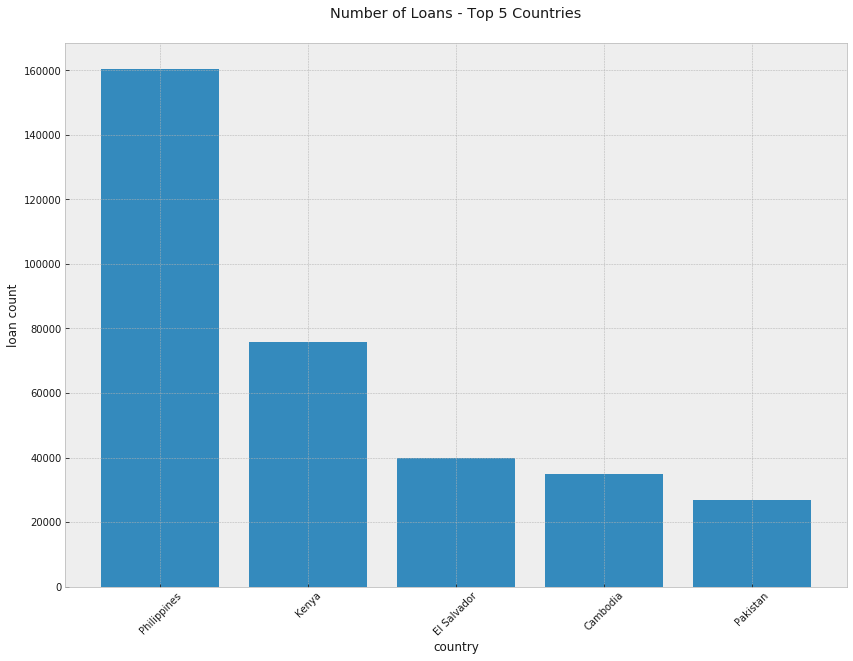
\includegraphics[width = 0.7 \textwidth]{loan_regions}
\end{figure}

As we can see, the Philippines is the region where Kiva mostly focuses their efforts in terms of loan count. Actually, when it comes to loan count, there are twice as many loans granted in the Philippines as in the second country in the list (Kenya).

Now we can focus on the Philippines and the FIES data. We will first derive an estimated family employment feature. It will be defined as: number of employed family members / (total number family members - children). We will also derive ‘no\_electricity’ and ‘no\_running\_water’ indicators.

Let's now plot the estimated family employment by region:

\begin{figure}[H]
\caption{Estimated Employment Per Region}
\centering
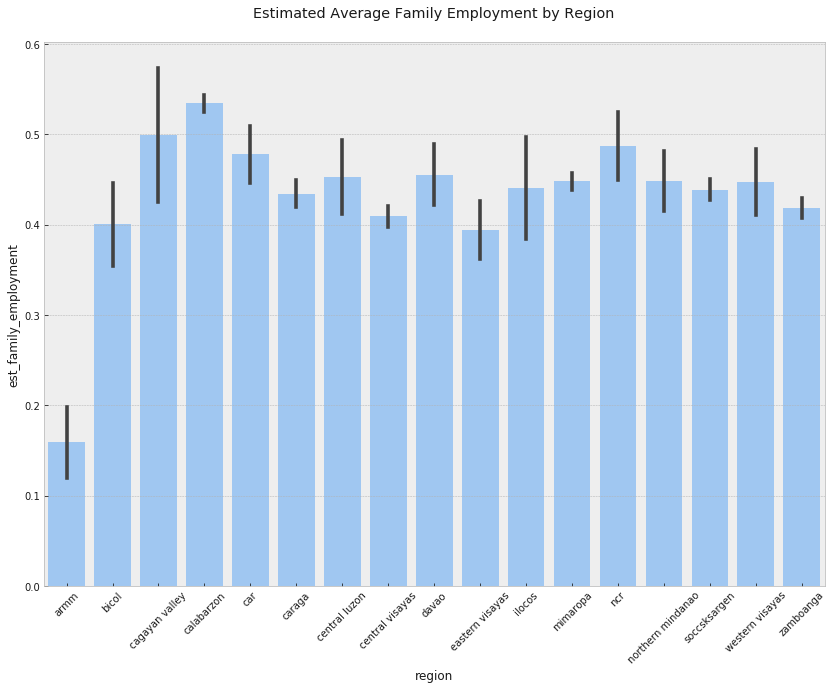
\includegraphics[width = 0.7 \textwidth]{empl_region}
\end{figure}

We can see from the very beginning that the Autonomous Region of Muslim Mindanao (ARMM) is severely affected by unemployment. Another notable feature is that in the Cagayan Valley the disparity in employment between households with male and female heads is greatest.

We continue by visualizing the three major poverty indicators (no running water, no toilet and no electricity):

\begin{figure}[H]
\caption{Poverty Indicators Per Region}
\centering
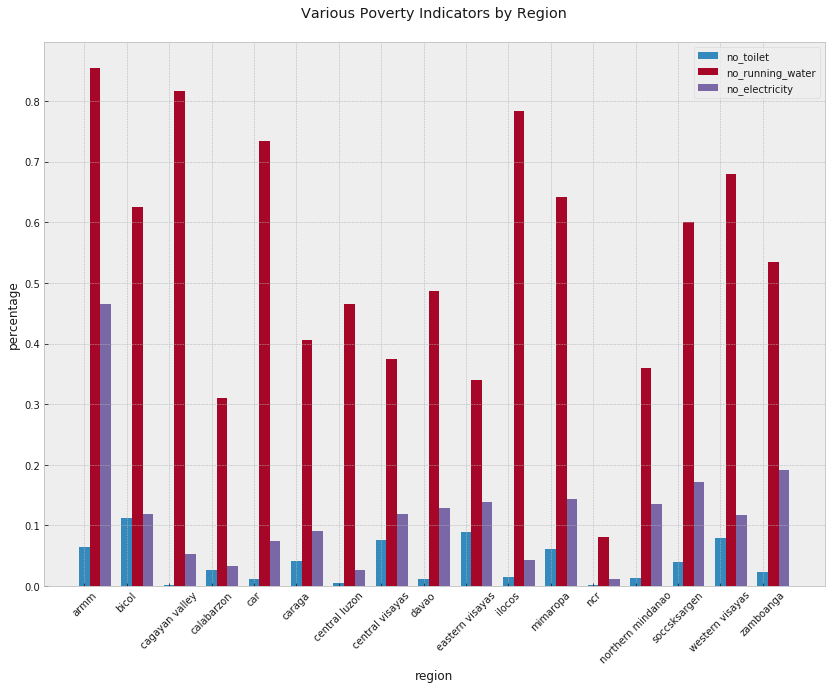
\includegraphics[width = 0.7 \textwidth]{poverty_indicators_region}
\end{figure}

Again ARMM is severely affected as measured by all three indicators. A good sense check of our data is the inspection of the corresponding values in the National Capital Regions (NCR). We should expect that there, the lack of infrastructure (running water, electricity and toilet) is the lowest. That is confirmed by the chart. We could also expect that incomes in the ARMM province would be the lowest for the country. Let's confirm that:

\begin{figure}[H]
\caption{Household Income Per Region}
\centering
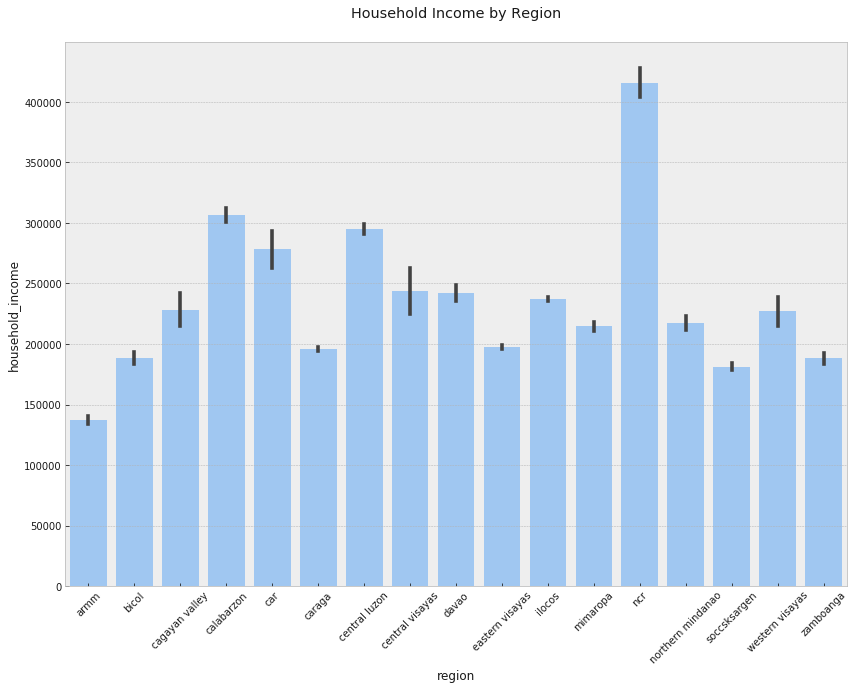
\includegraphics[width = 0.7 \textwidth]{household_income_region}
\end{figure}

The income distribution by region fits our expectations. Another observation (for the sake of sense-checking the data) is that the National Capital Region (NCR) has the highest average income. This is also in line with expectations.

We could expect that lack of communication means lack of access to the economy of the country. Let's investigate the relationship between the number of communication devices and household income in the next plot:

\begin{figure}[H]
\caption{Number of Communication Devices with Household Income}
\centering
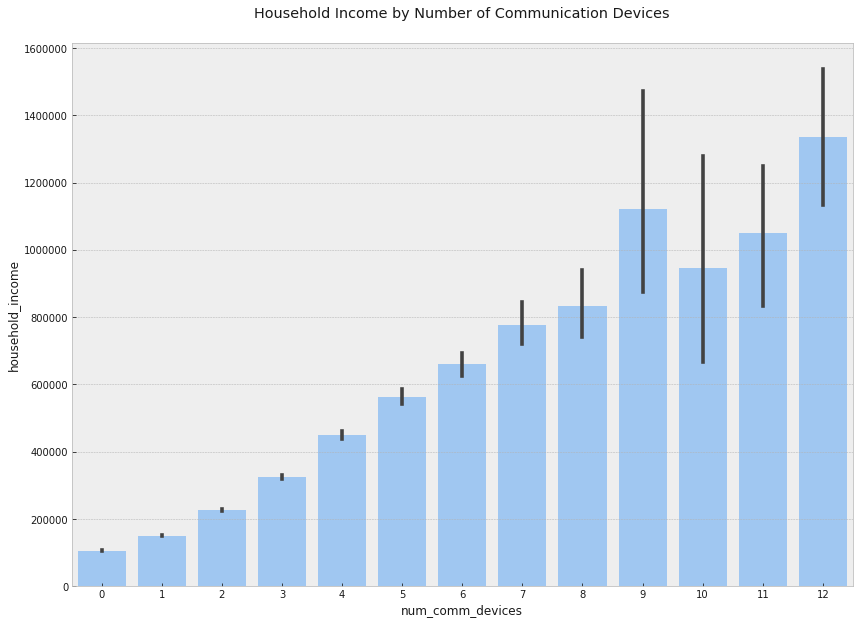
\includegraphics[width = 0.7 \textwidth]{household_income_comm_devices}
\end{figure}

Let's now turn to more general data patterns and investigate for useful predictors of income. We will start by comparing the distributions of food expenses and household income:

\begin{figure}[H]
\caption{Distribution of Food Expenses and Household Income}
\centering
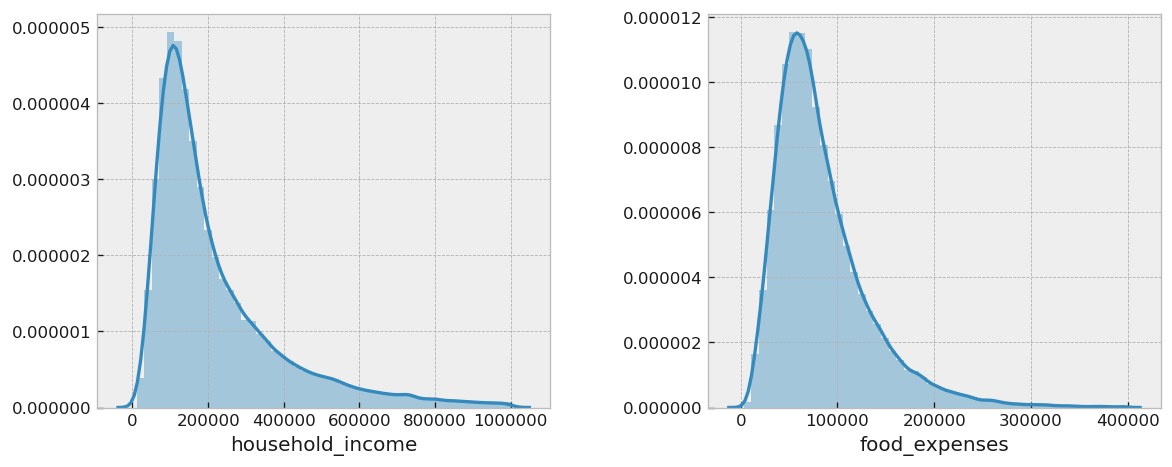
\includegraphics[width = 0.7 \textwidth]{food_expenses_income_dist}
\end{figure}

Apparently, the distributions are quite similar (both are positively skewed). We can visually inspect the correlation between the two variables in the next scatterplot:

\begin{figure}[H]
\caption{Household Income by Food Expenses}
\centering
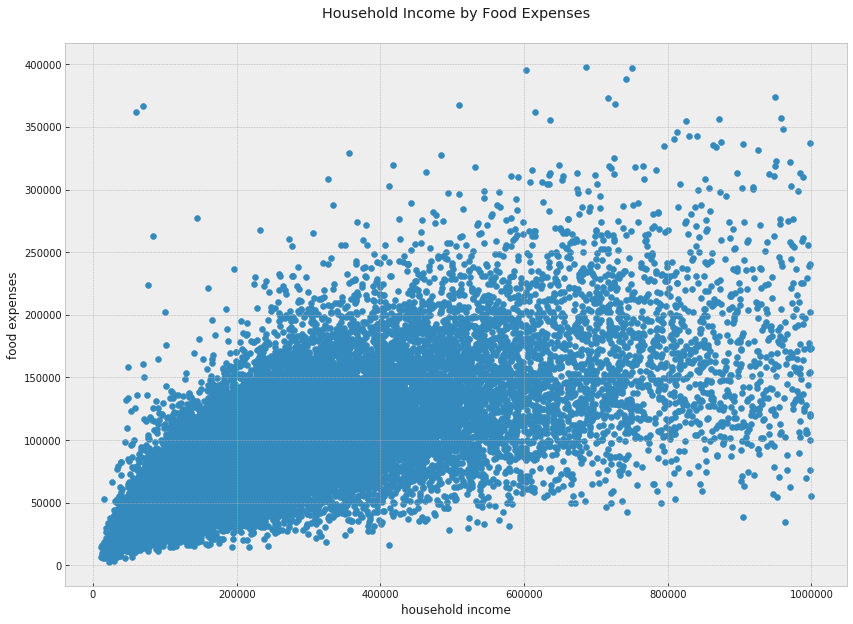
\includegraphics[width = 0.7 \textwidth]{household_income_food_expenses}
\end{figure}

There is an apparent correlation between household income and food expenses.

\subsection{Algorithms and Techniques}
%In this section, you will need to discuss the algorithms and techniques you intend to use for solving the problem. You should justify the use of each one based on the characteristics of the problem and the problem domain. Questions to ask yourself when writing this section:
%Are the algorithms you will use, including any default variables/parameters in the project clearly defined?
%Are the techniques to be used thoroughly discussed and justified?
%Is it made clear how the input data or datasets will be handled by the algorithms and techniques chosen?

We utilize the following data selection and transformation techniques in the poverty score’s modeling work:
\begin{itemize}
  \item Correlation inspection We use \href{http://pandas.pydata.org/pandas-docs/version/0.17.0/generated/pandas.DataFrame.corr.html}{Pandas implementation} of the Pearson correlation coefficient to inspect and reduce the number of input features to the model. The correlation coefficient is defined as:
    \begin{equation}
      r = \frac{n \sum x_i y_i - \sum x_i \sum y_i}{\sqrt{n \sum x_i^2 - (\sum x_i)^2} \sqrt{n \sum y_i^2 - (\sum y_i)^2}}
    \end{equation}
  \item Feature weight inspection: We use a model’s feature weight method in order to obtain the significance of the important features. This will allow us to reduce the number of new data that Kiva will need to obtain if they are to implement our model. Ideally, we have to reduce the number of features to 3-5 important questions that can be asked in the field.
  \item Normalization: As we saw in the visualization chapter, the household income distribution is positively skewed. On the other hand, there are many one hot encoded columns as explained in the Data Preprocessing chapter. This means that we will have data (such as the income and expenses) that will be overpowering the 0-1 one hot encoded indicators due to its scale. That’s why we need to apply a normalization on the dataset.
\end{itemize}

In our modeling work, we do not want to ignore any possibility for producing good results. That’s why we will use as many different model classes as possible. This will give us the opportunity to select the best performing model and tweak its parameters as well as the chance to use certain models’ idiosyncrasies (e.g. the decision tree model can be visualized, the linear regression model can be converted to a scorecard, etc.).  We utilize the following modelling algorithms:
\begin{itemize}
  \item AdaBoost Regressor: Boosting algorithms generally work well out of the box and we will use this one as representative from its class.
  \item Support Vector Machines Regressor: Support vector machines allow us to find data trends in higher dimensions and translate them back to our existing feature space.
  \item Stochastic Gradient Descent Regressor:
  \item Linear Regression: Linear regressions are simple and hold great explanatory power.
  \item Decision Tree Regressor: Decision trees can be visualized well and are not affected by outliers.
  \item Multi Layer Perceptron Regressor: This algorithm and its SciKit Learn implementation provide us with a quick and easy neural network class algorithm.
\end{itemize}

\subsection{Benchmark}
%In this section, you will need to provide a clearly defined benchmark result or threshold for comparing across performances obtained by your solution. The reasoning behind the benchmark (in the case where it is not an established result) should be discussed. Questions to ask yourself when writing this section:
%Has some result or value been provided that acts as a benchmark for measuring performance?
%Is it clear how this result or value was obtained (whether by data or by hypothesis)?
Since the normalized values for the household income have a range between 0 and 1, we will use 3 dummy predictors to evaluate the performance of our actual model against:
\begin{itemize}
  \item A dummy predictor that always predicts household income 0
  \item A dummy predictor that always predicts household income 1
  \item A dummy predictor that always predicts household income 0.5
\end{itemize}
We will evaluate these regressors based on our selected evaluation metrics and compare them to our actual model under development.

\section{Methodology}
%(approx. 3-5 pages)
\hypertarget{data_prep}{\subsection{Data Preprocessing}}
%In this section, all of your preprocessing steps will need to be clearly documented, if any were necessary. From the previous section, any of the abnormalities or characteristics that you identified about the dataset will be addressed and corrected here. Questions to ask yourself when writing this section:
%If the algorithms chosen require preprocessing steps like feature selection or feature transformations, have they been properly documented?
%Based on the Data Exploration section, if there were abnormalities or characteristics that needed to be addressed, have they been properly corrected?
%If no preprocessing is needed, has it been made clear why?
As we saw in the data exploration chapter, there are several preprocessing steps we have to take in order to make the data usable in our modeling task:
\begin{itemize}
  \item Map the Kiva loans region column to actual regions in the Philippines
  \item Transform the categorical fields from the FIES data to one hot encoded fields
  \item Give all columns query-friendly names
  \item Where necessary, reduce the categories of certain columns from the FIES data set
  \item Where necessary, merge certain columns from the FIES data set
  \item Normalize all columns from the FIES data sets
\end{itemize}
Here, we’ll describe in detail the pre-processing of both the Kiva loans and the FIES data sets.

\subsubsection{Kiva Loans Data Set Transformation}
Let us first lay out the administrative region hierarchy of the Philippines:

\begin{enumerate}
  \item Island Group
  \item Region
  \item Province
  \item City
\end{enumerate}

For most of the cases (about 145000 out of 160000), the ‘region’ column from the Kiva loans data set contains a pattern of the type: ‘city name, province’. We can make a supplementary matching table with the administrative region types as columns and the administrative region names as rows. We will then separate each ‘city name, province’ entry into city name and province name. We will then use the province name to match the actual Region in the Philippines.

Here is an example of a few rows from our matching table:

\begin{center}
\begin{tabular}{ |l|l|l|l| }
  \hline
  island\_group & region & province & city\\
  \hline
  luzon & ilocos & ilocos norte & laoag\\
  luzon & ilocos & ilocos sur & vigan\\
  luzon & ilocos & la union & san fernando\\
  luzon & ilocos & pangasinan & lingayen\\
  luzon & cagayan valley & batanes & basco\\
  luzon & cagayan valley & cagayan & tuguegarao city\\
  luzon & cagayan valley & isabela & ilagan\\
  \hline
\end{tabular}
\end{center}

If we have the following entry from the Kiva loans data set: ‘laoag, ilocos norte’, we will separate it into ‘laoag’ and ‘ilocos norte’, take the province name of ‘ilocos norte’ and look up what is its adjacent region (in this case ‘ilocos’). That means that our matching algorithm for the bulk of the entries is:

\begin{enumerate}
  \item Convert all names to lowercase
  \item For each entry in the ‘region’ column from the Kiva loans data set:
  \begin{itemize}
    \item Split the entry into city and province
    \item Take the province
    \item Match the province with a region from the matching table using Python’s built-in ‘get\_close\_matches’ method
    \item Return the region from the matching table
  \end{itemize}
\end{enumerate}

For the cases where this method is unsuccessful (15000 cases), we will attempt to match the city name. We will do that by using the algorithm above, but matching against the city instead of the province. This helps us match further 5000 entries from the Kiva loans table.

We will discard all entries that have missing value, no major population center listed or have unclear location (about 10000 rows).

\subsubsection{FIES Data Set Transformation}
There is one general transformation that all columns need to undergo: renaming them to query-friendly names. In addition, before one hot encoding, all categorical string values will also be mapped to query-friendly names as those values will become one hot encoded columns themselves. It is worth describing our query-friendly naming convention:

\begin{itemize}
  \item All words are in lowercase
  \item There are no spaces, words are separated by an underscore (‘\_’)
  \item Where possible, words are abbreviated
\end{itemize}

Here is one example of converting a column name: 'Members with age less than 5 year old' \\ becomes 'num\_children\_younger\_5'. Here is an example of categorical string values mapping (for the 'Type of Household' column): the value 'Extended Family' is mapped to 'house\_ext\_family'. When one hot encoded, the value 'house\_ext\_family' will become a column itself containing the values 1 and 0.

Let us now go over all transformed columns and describe their transformations in detail:

\begin{itemize}
  \item Region: the values are mapped to a common naming convention shared by the Kiva loans data set.
  \item The columns: 'Bread and Cereals Expenditure', 'Total Rice Expenditure', 'Meat Expenditure', 'Total Fish and  marine products Expenditure', 'Fruit Expenditure', 'Vegetables Expenditure' are removed (only the ‘food\_expenses’ column is used instead).
  \item The values of the columns: 'Restaurant and hotels Expenditure', 'Alcoholic Beverages Expenditure', 'Tobacco Expenditure' are summed into the 'non\_essential\_expenses' column. The columns: 'Restaurant and hotels Expenditure', 'Alcoholic Beverages Expenditure', 'Tobacco Expenditure' are then removed from the data set.
  \item The categorical string values from the 'Household Head Sex' column are mapped to: 'Female' : 1 and 'Male' : 0. The column is then renamed to: 'house\_head\_sex\_f'.
  \item The column 'Household Head Marital Status' contains various categorical string values such as: 'Single', 'Widowed', 'Divorced/Separated', 'Annulled', 'Unknown', ‘Married’, etc. We will reduce these statuses to 2 values: 'house\_head\_single' and 'house\_head\_partner'. This is because for the purpose of household income estimation, what matters is if there are two income earners in the household or just one. We will then one hot encode the column and drop it.
  \item The 'Household Head Highest Grade Completed' contains many statuses corresponding to each possible grade of school completed as well as to all possible university majors. This is quite an extensive list, but for the purpose of income estimation, only the education level matters (e.g. a person with university education will definitely earn more than an illiterate person). That’s why we will group all values into: 'house\_head\_illiterate', 'house\_head\_primary\_ed', 'house\_head\_secondary\_ed', 'house\_head\_tertiary\_ed'. We will then one hot encode these grouped values and drop the column.
  \item The column 'Household Head Job or Business Indicator' can be renamed to 'house\_head\_empl' and the values can be mapped as: 'With Job/Business' : 1, 'No Job/Business' : 0.
  \item The 'Household Head Occupation' column contains over 300 values. This is too specific and will unnecessary complicate our data set if one hot encoded. Besides many job types are more or less duplicates (e.g. ‘General Manager in the Hospitality Industry’ and ‘General Manager in the Textile Industry’). On the other hand, our ultimate goal is to be able to estimate poverty levels. With regards to that, we can derive a flag for all professions that are related to farming. Our intuition is that in the context of poverty assessment, the farming professions would be meaningful. The rationale behind that is that farmers are usually the most isolated and poor individuals, especially in developing countries. We'll use a simple regular expression to derive the farming professions and map them to a 'house\_head\_farmer\_flag'.
  \item For the columns: ‘Type of Household’, ‘Type of Building/House’, ‘Main Source of Income’, 'Type of Roof', 'Type of Walls' and 'Toilet Facilities': the categorical values are mapped to query-friendly names and one hot encoded.
  \item The column 'Main Source of Water Supply' is reduced to an indicator of 'running\_water'. The indicator has values 1 and 0.
  \item The values of the columns: 'Number of Television', 'Number of CD/VCD/DVD', 'Number of Component/Stereo set', 'Number of Personal Computer' are summed into the column 'num\_electronics'. The columns: 'Number of Television', 'Number of CD/VCD/DVD', 'Number of Component/Stereo set', 'Number of Personal Computer' are then removed from the data set.
  \item The values of the columns: 'Number of Landline/wireless telephones' and  'Number of Cellular phone' are summed into the column 'num\_comm\_devices'. We are summing those two columns into a separate feature from the 'num\_electronics' because poverty is also related to lack of access to communications and to the financial system. It is apparent (as shown in the Visualization chapter) that lack of communication is a meaningful feature and should be derived on its own. The columns:  'Number of Landline/wireless telephones' and  'Number of Cellular phone' are then removed from the data set.
  \item The columns: 'Number of Car, Jeep, Van', 'Number of Motorized Banca', 'Number of Motorcycle/Tricycle' are summed into the column 'num\_vehicles'. The columns 'Number of Car, Jeep, Van', 'Number of Motorized Banca', 'Number of Motorcycle/Tricycle' are then dropped from the data set.
  \item All remaining columns are renamed to query-friendly names.
\end{itemize}

As an additional step to our modeling, we will also normalize the so transformed FIES data set. So that skewing or uneven scaling of the data won’t affect the performance of our models.

\subsubsection{Data Selection}
As a final step in our preprocessing we need to inspect the various feature correlations. We will start with columns from the FIES data set which have similar meaning to the original target variable. There are several columns that would correlate highly with the 'household\_income' column. Those are:

\begin{itemize}
  \item 'income\_from\_entrepreneur\_activities'
  \item 'main\_inc\_entrepreneur'
  \item 'main\_inc\_other'
  \item 'main\_inc\_wage'
\end{itemize}

Let's see the actual correlation levels and confirm that:

\begin{center}
\resizebox{\textwidth}{!}{%
\begin{tabular}{ |l|l|l|l|l|l| }
  \hline
  feature & household\_income & income\_from\_entrepreneur\_activities 1 & main\_inc\_entrepreneur & main\_inc\_other & main\_inc\_wage\\
  \hline
  household\_income & 1 & 0.563662 & -0.068279 & -0.010181 & 0.067958 \\
  income\_from\_entrepreneur\_activities & 0.563662 & 1 & 0.363651 & -0.106587 & -0.220697 \\
  main\_inc\_entrepreneur & -0.068279 & 0.363651 & 1 & -0.341511 & -0.564373 \\
  main\_inc\_other & -0.010181 & -0.106587 & -0.341511 & 1 & -0.583149 \\
  main\_inc\_wage & 0.067958 & -0.220697 & -0.564373 & -0.583149 & 1 \\
  \hline
\end{tabular}}
\end{center}

Here is a visualization of the table above:

\begin{figure}[H]
\caption{Correlation Matrix - Income Features}
\centering
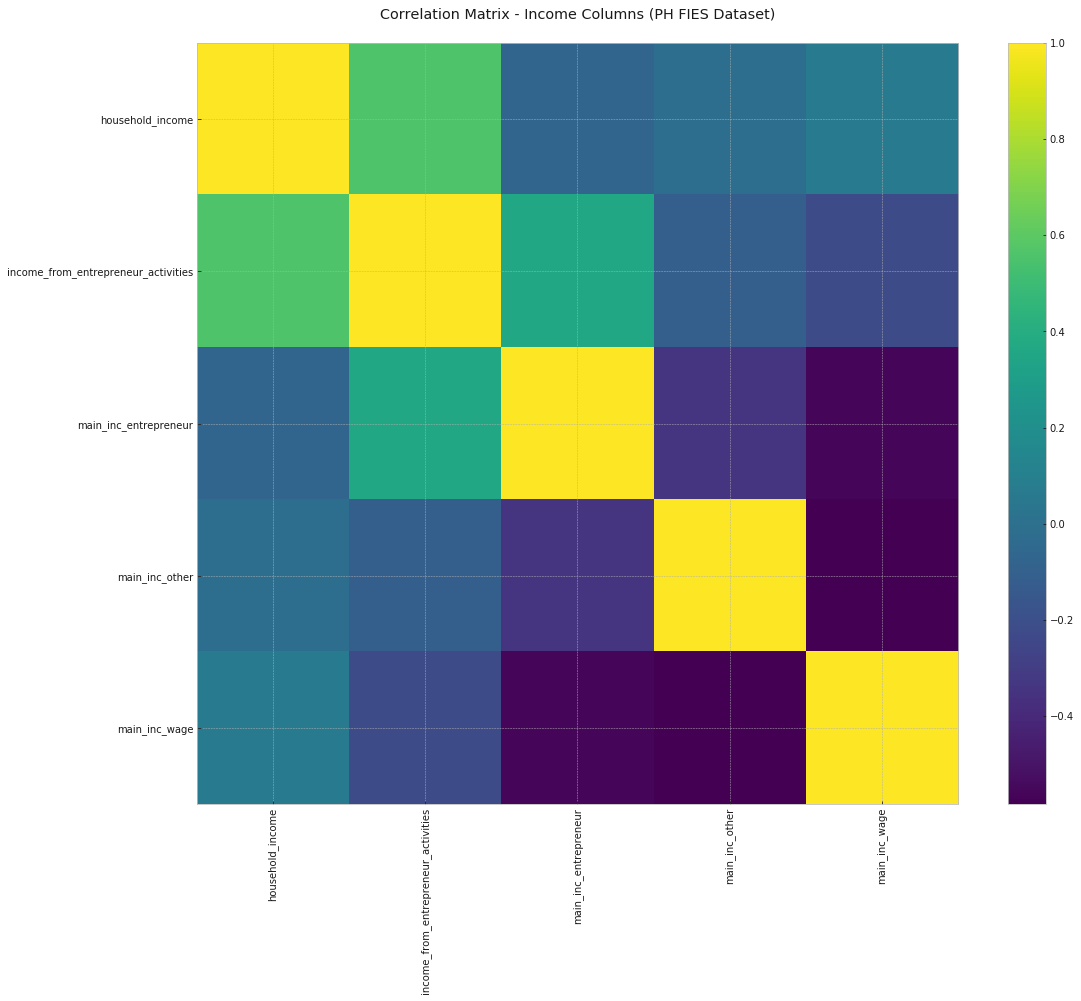
\includegraphics[width = 0.7 \textwidth]{income_corr_matrix}
\end{figure}

As we can see, there is a high correlation between the various income columns and the ‘household\_income’ target. That’s why we have to remove these columns from the data set.

We can now plot all remaining variables and visually inspect for any other correlation patterns:

\begin{figure}[H]
\caption{Correlation Matrix - All Features}
\centering
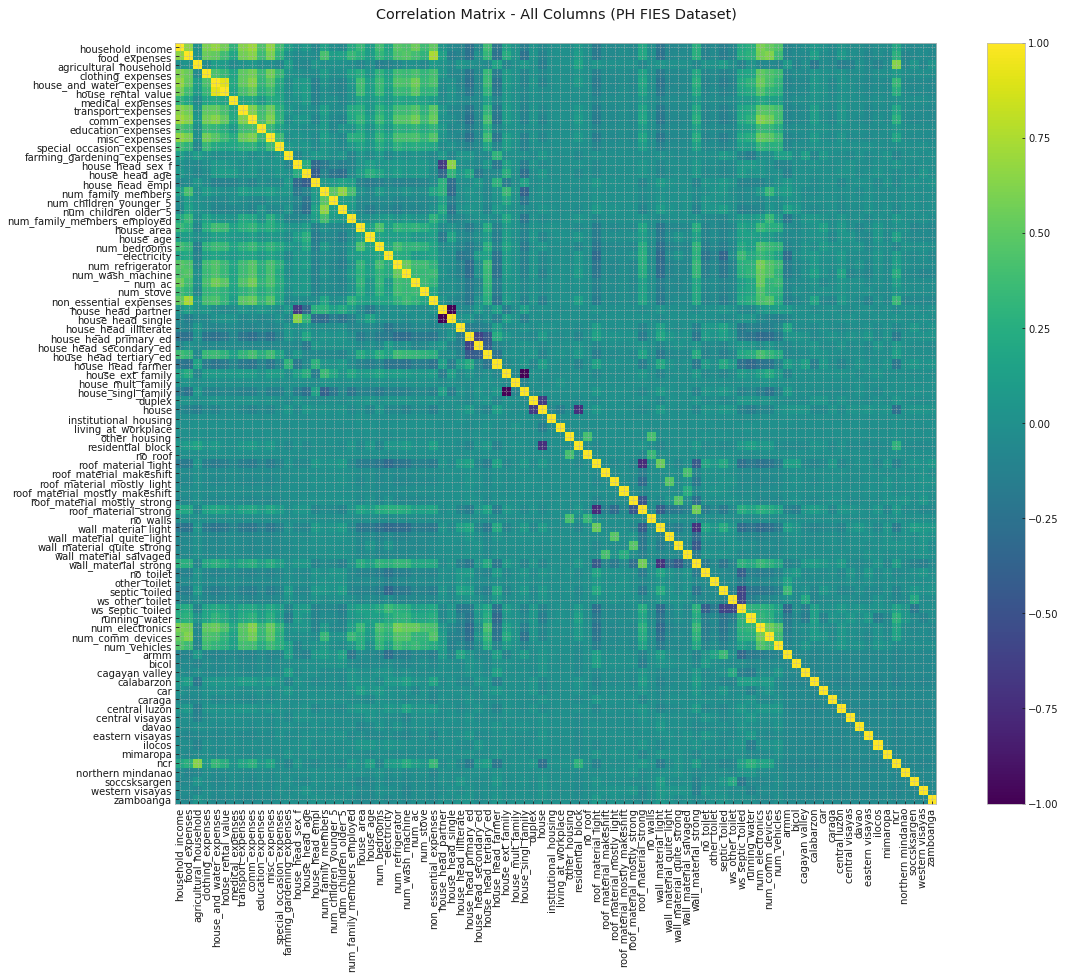
\includegraphics[width = 0.7 \textwidth]{all_features_corr_1}
\end{figure}

As we can see, there are some high positive and some inverse correlations. Let's zoom in on several examples:

\begin{itemize}
  \item The expenses columns seem to correlate highly with one another. That is reasonable as high 'transportation' or 'other' expenses indicate an affluent household. We could expect such a household to also have high 'clothing' expenses.
  \item There are some inversely-correlated columns (e.g. house\_head\_single and house\_head\_parther). The relationship there is more than obvious - if the house head is single, they definitely don't have a partner.
  \item The household\_income column seems to correlate highly with the following fields:
  \begin{itemize}
    \item Expenses (food expenses, clothing expenses, house and water expenses, transport expenses, communication expenses and miscellaneous expenses)
    \item House rental value
    \item Number of ACs (air conditioning appliances)
    \item Number of electronic devices (DVDs, CD, stereo, etc.)
    \item Number of communication devices (landline or mobile phones)
    \item Number of vehicles (cars, tricycles, motorized boats)
  \end{itemize}
\end{itemize}

Those correlations seem to reasonably point towards the welfare of individuals. After all, poverty is not only the lack of disposable income, but also exclusion through lack of connectivity, transportation and financing.

At this point, we will:

\begin{itemize}
  \item Visualize the correlation of the expenses features:
  \begin{itemize}
    \item food\_expenses
    \item clothing\_expenses
    \item house\_and\_water\_expenses
    \item medical\_expenses
    \item transport\_expenses
    \item comm\_expenses
    \item education\_expenses
    \item misc\_expenses
    \item special\_occasion\_expenses
    \item farming\_gardening\_expenses
    \item non\_essential\_expenses
  \end{itemize}
  \item Remove one of each inversely-correlating pairs
  \item Remove the non-relevant expenses. The reason for that is to make the model less reliant on information from the same category. This will also allow us to require less data if we scale the model internationally (it will be way easier to find food expenses data alone than food, clothing, miscellaneous, transportation, etc. together).
\end{itemize}

\begin{center}
\resizebox{\textwidth}{!}{%
\begin{tabular}{ |l|l|l|l|l|l|l|l|l|l|l|l| }
  \hline
  feature & food\_expenses & clothing\_expenses & house\_and\_water\_expenses & medical\_expenses & transport\_expenses & comm\_expenses & education\_expenses & misc\_expenses & special\_occasion\_expenses & farming\_gardening\_expenses & non\_essential\_expenses\\
  \hline
  food\_expenses & 1 & 0.543237 & 0.522252 & 0.186645 & 0.577372 & 0.633819 & 0.374898 & 0.594453 & 0.296624 & 0.0208 & 0.744933\\
  clothing\_expenses & 0.543237 & 1 & 0.432092 & 0.172845 & 0.503026 & 0.574041 & 0.34377 & 0.565225 & 0.337542 & 0.04438 & 0.401855\\
  house\_and\_water\_expenses & 0.522252 & 0.432092 & 1 & 0.212181 & 0.515797 & 0.639698 & 0.327944 & 0.470872 & 0.216761 & -0.01216 & 0.429699\\
  medical\_expenses & 0.186645 & 0.172845 & 0.212181 & 1 & 0.20037 & 0.214714 & 0.088768 & 0.231703 & 0.185885 & 0.010141 & 0.113158\\
  transport\_expenses & 0.577372 & 0.503026 & 0.515797 & 0.20037 & 1 & 0.621611 & 0.386692 & 0.54453 & 0.272043 & 0.050873 & 0.491167\\
  comm\_expenses & 0.633819 & 0.574041 & 0.639698 & 0.214714 & 0.621611 & 1 & 0.419618 & 0.604349 & 0.293515 & -0.005839 & 0.533568\\
  education\_expenses & 0.374898 & 0.34377 & 0.327944 & 0.088768 & 0.386692 & 0.419618 & 1 & 0.334283 & 0.15884 & 0.035074 & 0.315932\\
  misc\_expenses & 0.594453 & 0.565225 & 0.470872 & 0.231703 & 0.54453 & 0.604349 & 0.334283 & 1 & 0.371388 & 0.013091 & 0.458687\\
  special\_occasion\_expenses & 0.296624 & 0.337542 & 0.216761 & 0.185885 & 0.272043 & 0.293515 & 0.15884 & 0.371388 & 1 & 0.074255 & 0.180372\\
  farming\_gardening\_expenses & 0.0208 & 0.04438 & -0.01216 & 0.010141 & 0.050873 & -0.005839 & 0.035074 & 0.013091 & 0.074255 & 1 & -0.04078\\
  non\_essential\_expenses & 0.744933 & 0.401855 & 0.429699 & 0.113158 & 0.491167 & 0.533568 & 0.315932 & 0.458687 & 0.180372 & -0.04078 & 1\\
  \hline
\end{tabular}}
\end{center}

Here is a visualization of the correlation matrix:

\begin{figure}[H]
\caption{Correlation Matrix - Expenses Features}
\centering
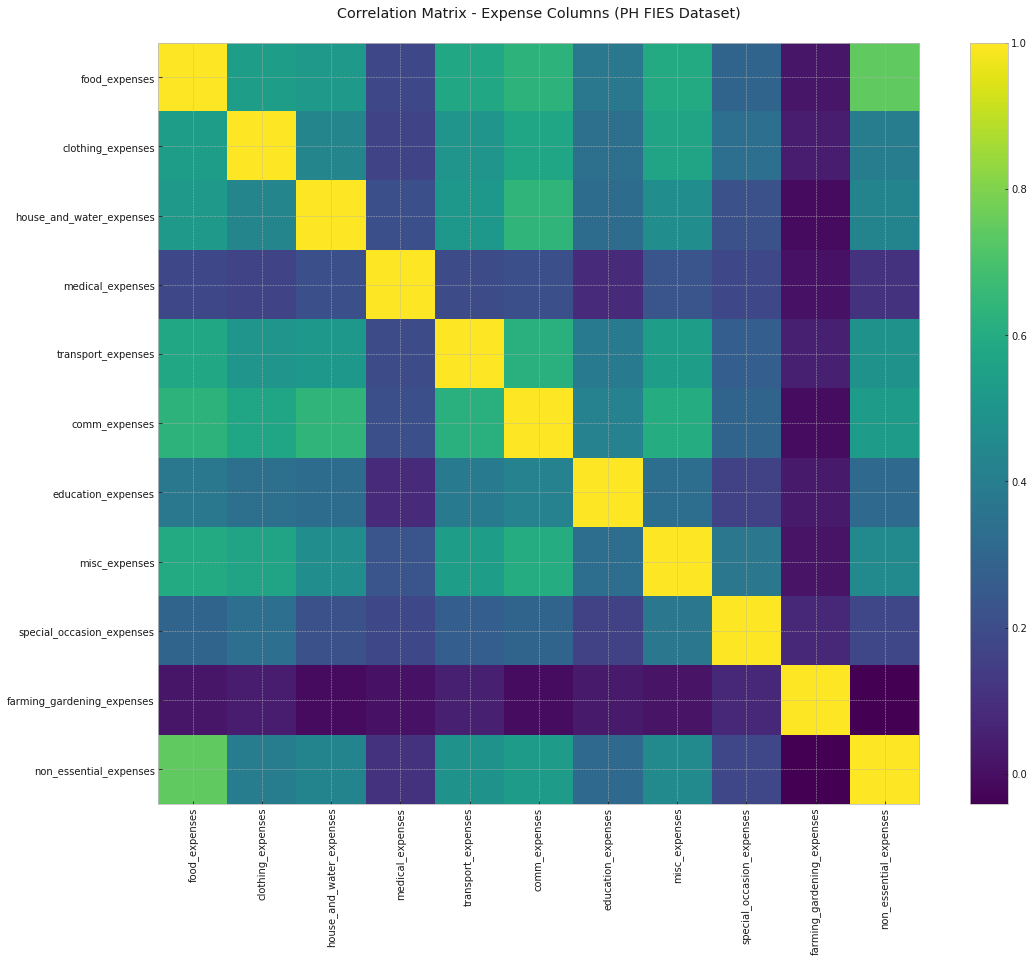
\includegraphics[width = 0.7 \textwidth]{expenses_corr_matrix}
\end{figure}

We will remove all expense columns except the ‘food\_expenses’. Here is a visualization of the correlation between the remaining features:

\begin{figure}[H]
\caption{Correlation Matrix - All Features}
\centering
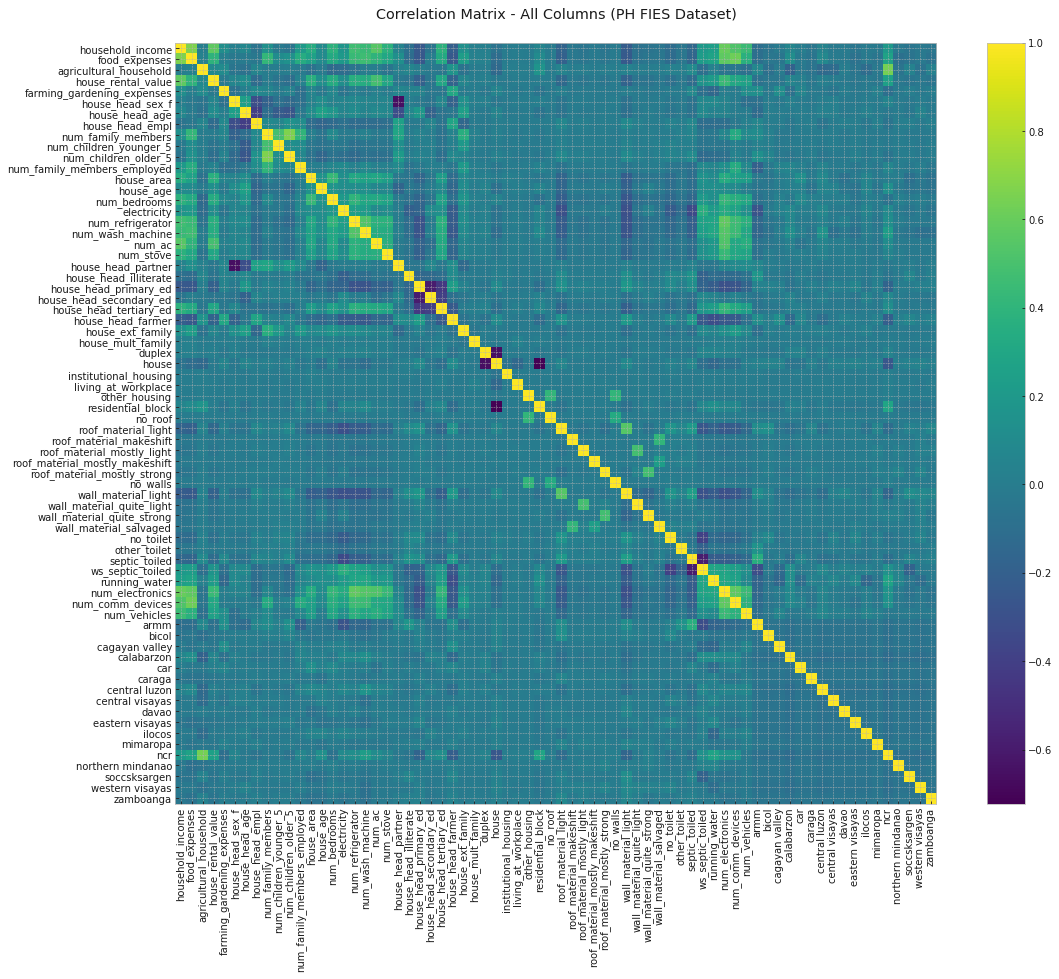
\includegraphics[width = 0.7 \textwidth]{all_features_corr_2}
\end{figure}

\subsection{Implementation}
%In this section, the process for which metrics, algorithms, and techniques that you implemented for the given data will need to be clearly documented. It should be abundantly clear how the implementation was carried out, and discussion should be made regarding any complications that occurred during this process. Questions to ask yourself when writing this section:
%Is it made clear how the algorithms and techniques were implemented with the given datasets or input data?
%Were there any complications with the original metrics or techniques that required changing prior to acquiring a solution?
%Was there any part of the coding process (e.g., writing complicated functions) that should be documented?

At this point, we can derive an initial model. We'll use that model and its highest-performing features in order to reduce the number of input columns later on.

We will separate the data into a training and testing sets. We will only use the training set with cross validation in order to select the best fields. We will then use the test set to evaluate the final model's performance. The specific steps we will p

\begin{enumerate}
  \item Scaling and normalizing the data
  \item Dividing the data into a training and testing sets
  \item Evaluating an initial model (out of all the candidates described in the Algorithms section)
  \item Selecting the columns with the highest weights
  \item Creating the final model
  \item Measuring the model's performance
\end{enumerate}

We will train and validate several model types without any tweaking. We'll do that on portions of the training dataset. We'll then produce some performance metrics that will allow us to focus on one or two of the models. For the purpose of benchmarking, we will also include validation results for three dummy regressors that always predict 0, 0.5 and 1 respectively:

\begin{center}
\begin{tabular}{ |l|l|l|l|l| }
  \hline
  regressor & mean\_squared\_error & r2\_score & mean\_squared\_log\_error & explained\_variance\_score \\
  \hline
  ada\_boost & 0.000585 & 0.881831 & 1.62E-04 & 8.89E-01\\
  svr & 0.006065 & -0.224031 & 1.75E-03 & 8.13E-01\\
  sgd & 0.001681 & 0.660628 & 5.07E-04 & 6.61E-01\\
  decision\_tree & 0.000024 & 0.99521 & 8.00E-06 & 9.95E-01\\
  linear & 0.000425 & 0.914236 & 1.32E-04 & 9.14E-01\\
  mlp & 0.000156 & 0.968477 & 5.30E-05 & 9.68E-01\\
  dummy\_0.0 & 0.797975 & -160.057695 & 4.06E-01 & 0.00E+00\\
  dummy\_0.5 & 0.157458 & -30.780255 & 0.054666 & 0.00E+00\\
  dummy\_1 & 0.016941 & -2.419269 & 0.004708 & -2.22E-16\\
  \hline
\end{tabular}
\end{center}

As we can see, the Decision Tree and the Multi Level Perceptron regressor, the Linear regression and AdaBoost regressor are performing best out of the box. All of them outperform the dummy regressors in all metrics by a significant margin.

Let's look the top 4 models’ feature importances (or in the case of the Linear Regression and the Multi Layer Perceptron regressor, the feature coefficients):

\begin{multicols}{2}
AdaBoost regressor
\begin{flushleft}
\begin{tabular}{ |l|l| }
  \hline
  feature & importance\\
  \hline
  food\_expenses & 0.744377\\
  farming\_gardening\_expenses & 0.198619\\
  house\_rental\_value & 0.047395\\
  agricultural\_household & 0.006434\\
  house\_area & 0.001426\\
  house\_head\_partner & 0.00063\\
  house & 0.000366\\
  armm & 0.000361\\
  house\_head\_empl & 0.000353\\
  num\_electronics & 0.000039\\
  \hline
\end{tabular}
\end{flushleft}
Decision Tree regressor
\begin{flushleft}
\begin{tabular}{ |l|l| }
  \hline
  feature & importance\\
  \hline
  food\_expenses & 0.632135\\
  farming\_gardening\_expenses & 0.348987\\
  house\_rental\_value & 0.016567\\
  house & 0.001125\\
  house\_head\_partner & 0.000141\\
  num\_comm\_devices & 0.000097\\
  house\_head\_primary\_ed & 0.000077\\
  agricultural\_household & 0.000073\\
  num\_bedrooms & 0.000063\\
  num\_electronics & 0.00006\\
  \hline
\end{tabular}
\end{flushleft}
Linear Regression
\begin{flushleft}
\begin{tabular}{ |l|l| }
  \hline
  feature & importance\\
  \hline
  no\_roof & 2257.82356\\
  ncr & 750.759429\\
  car & 694.030488\\
  zamboanga & 669.26106\\
  duplex & 536.816816\\
  other\_toilet & 509.406187\\
  num\_refrigerator & 471.154704\\
  davao & 469.813611\\
  house & 466.653182\\
  residential\_block & 434.85659\\
  \hline
\end{tabular}
\end{flushleft}
MLP regressor
\begin{flushleft}
\begin{tabular}{ |l|l| }
  \hline
  feature & importance\\
  \hline
  farming\_gardening\_expenses & 0.133671\\
  house\_area & 0.082551\\
  food\_expenses & 0.0688\\
  num\_children\_older\_5 & 0.054415\\
  num\_comm\_devices & 0.046787\\
  num\_electronics & 0.027852\\
  house\_head\_empl & 0.02675\\
  house\_head\_partner & 0.006638\\
  running\_water & 0.004642\\
  house\_head\_primary\_ed & 0.003707\\
  \hline
\end{tabular}
\end{flushleft}
\end{multicols}

We can draw some conclusions the feature importance rankings, namely:

\begin{itemize}
  \item The food\_expenses variable has the highest weight in both the AdaBoost and the Decision Tree models. This seems to be reasonable as low income families have predominantly food expenses that they need to limit due to their situation.
  \item The farming\_gardening\_expenses has the second highest weight in both the AdaBoost and the Decision Tree models. This is also is in line with the general reasoning for poor households - they are mostly rural and within farming communities. Actually the Kiva dataset for loan themes contains a rural percentage column (supposedly for the same reason).
  \item There are other important indicators of poverty which also seem in line with our intuition. Such are:
  \begin{itemize}
    \item Number of communication devices (or lack thereof)
    \item Agricultural household indicator
    \item House area
    \item House head employment status
    \item House head having partner indicator
    \item Number of family members
  \end{itemize}
\end{itemize}

It's also interesting to note that the Linear Regression has placed high importance on the regions and the living conditions (the no\_roof, other\_toilet, num\_refrigerator). Unfortunately we cannot simply use the region features because that would make the model harder to scale in the future (such a model will be basically a map of poverty-stricken regions).

The MLP regressor (at least in one of the dimensions if its matrix) has selected a mix of features, namely:

\begin{itemize}
  \item Expenses: farming\_gardening\_expenses
  \item Demographics: num\_children\_older\_5, house\_head\_secondary\_ed, house\_head\_tertiary\_ed
  \item Living conditions: house\_ext\_family, wall\_material\_quite\_light, residential\_block, roof\_material\_light
  \item Region: armm (as we saw in the Visualization chapter, this is the poorest region in the Philippines)
\end{itemize}

Here, we have some features that we can work with and some features that would be difficult to implement. One aspect of the MLP regressor that is disadvantageous for us is the difficulty in understanding its decision matrix (let's remember that these are the weights of just one perceptron out of 100 in the first layer). At least we get a partial confirmation that the food\_expenses column is a very important feature.

\subsection{Refinement}
%In this section, you will need to discuss the process of improvement you made upon the algorithms and techniques you used in your implementation. For example, adjusting parameters for certain models to acquire improved solutions would fall under the refinement category. Your initial and final solutions should be reported, as well as any significant intermediate results as necessary. Questions to ask yourself when writing this section:
%Has an initial solution been found and clearly reported?
%Is the process of improvement clearly documented, such as what techniques were used?
%Are intermediate and final solutions clearly reported as the process is improved?
Having a better understanding of the feature importances, the successful initial models and the validity of our approach, we can now proceed and derive the final model. To do that, we will:

\begin{enumerate}
  \item Select the model
  \item Select 3 features based on the following criteria:
  \begin{itemize}
    \item Feature weight
    \item Feature applicability (how easy would be for Kiva to integrate such a question into their loan application form)
  \end{itemize}
  \item Retrain the model on the selected features.
  \item Test the model performance on the test set.
\end{enumerate}

We'll start first by selecting the model. Based on the performance table, derived above, it would seem reasonable to select the Decision Tree model. Another good reason for choosing it is that decision trees are easily explainable.

Next, we move on the the 3 features. Our choice is: food\_expenses, farming\_gardening\_expenses and agricultural\_household. We prefer the agricultural\_household feature as it seems easier to apply in the field, however its weight is less than 1\% of our model's prediction power, so we can drop it altogether.

We'll now assess the performance after retraining (we are expecting a slight drop in performance because we limited ourselves to 2 features):

\begin{center}
\begin{tabular}{ |l|l| }
  \hline
  metric & value\\
  \hline
  mean\_squared\_error\_test & 0.000203\\
  r2\_score\_test & 0.961063\\
  mean\_squared\_log\_error\_test & 0.000056\\
  explained\_variance\_score\_test & 0.961064\\
  \hline
\end{tabular}
\end{center}

\section{Results}
%(approx. 2-3 pages)
\subsection{Model Evaluation and Validation}
%In this section, the final model and any supporting qualities should be evaluated in detail. It should be clear how the final model was derived and why this model was chosen. In addition, some type of analysis should be used to validate the robustness of this model and its solution, such as manipulating the input data or environment to see how the model’s solution is affected (this is called sensitivity analysis). Questions to ask yourself when writing this section:
%Is the final model reasonable and aligning with solution expectations? Are the final parameters of the model appropriate?
%Has the final model been tested with various inputs to evaluate whether the model generalizes well to unseen data?
%Is the model robust enough for the problem? Do small perturbations (changes) in training data or the input space greatly affect the results?
%Can results found from the model be trusted?
We can now combine all predictions and derive the poverty score from the predicted normalized income. In the future, as we add more countries to the estimation, our poverty score will more and more reflect global levels. Here is an initial distribution description of our poverty score:

\begin{center}
\begin{tabular}{ |l|l|l| }
  \hline
  metric &  predicted income & poverty score\\
  \hline
  count & 41544 & 41544\\
  mean & 0.890068 & 0.109932\\
  std & 0.071839 & 0.071839\\
  min & 0.103609 & 0.000511\\
  25\% & 0.853509 & 0.056976\\
  50\% & 0.903322 & 0.096678\\
  75\% & 0.943024 & 0.146491\\
  max & 0.999489 & 0.896391\\
  \hline
\end{tabular}
\end{center}

We will now join the region and house head female indicators from the original FIES data set. This will allow us to merge the poverty score with the Kiva loans data based on region and gender (as prescribed by the rules of the Kiva challenge). We will then provide visualizations for the results in the next chapter.

\subsection{Justification}
%In this section, your model’s final solution and its results should be compared to the benchmark you established earlier in the project using some type of statistical analysis. You should also justify whether these results and the solution are significant enough to have solved the problem posed in the project. Questions to ask yourself when writing this section:
%Are the final results found stronger than the benchmark result reported earlier?
%Have you thoroughly analyzed and discussed the final solution?
%Is the final solution significant enough to have solved the problem?

As we saw in the initial tests, the results of the dummy predictors (our chosen benchmarks) and our final model were (note that here the final model's metrics are on the test set):

\begin{center}
\begin{tabular}{ |l|l|l|l|l| }
  \hline
  regressor & mean squared error & r2 score & mean squared log error & explained variance score\\
  \hline
  dummy\_0.0 & 0.797975 & -160.057695 & 4.06E-01 & 0.00E+00\\
  dummy\_0.5 & 0.157458 & -30.780255 & 0.054666 & 0.00E+00\\
  dummy\_1 & 0.016941 & -2.419269 & 0.004708 & -2.22E-16\\
  final model on test set & 0.000203 & 0.961063 & 0.000056 & 0.961064\\
  \hline
\end{tabular}
\end{center}

It seems that our final model generalizes well on unseen data.

\section{Conclusion}
%(approx. 1-2 pages)
\subsection{Free-Form Visualization}
%In this section, you will need to provide some form of visualization that emphasizes an important quality about the project. It is much more free-form, but should reasonably support a significant result or characteristic about the problem that you want to discuss. Questions to ask yourself when writing this section:
%Have you visualized a relevant or important quality about the problem, dataset, input data, or results?
%Is the visualization thoroughly analyzed and discussed?
%If a plot is provided, are the axes, title, and datum clearly defined?

Let us now visualize the distribution of the poverty score by region and gender:

\begin{figure}[H]
\caption{Poverty Score by Region and Gender}
\centering
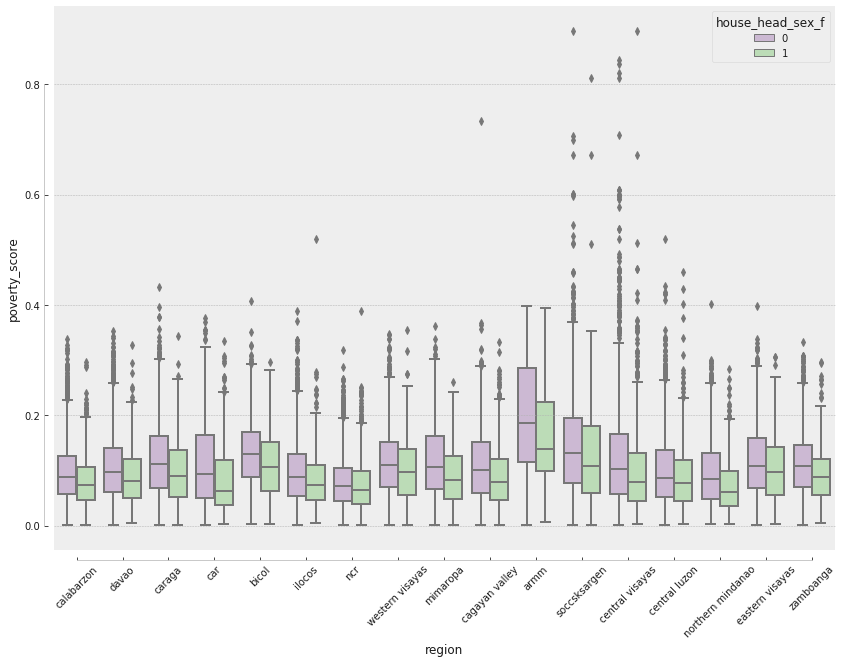
\includegraphics[width = 0.7 \textwidth]{poverty_score_region_gender}
\end{figure}

As we can see, the Visayas Island, the Soccsksargen province and the Administrative Region of Muslim Mindanao score consistently high in poverty score, compared to other regions. The interesting thing about Visayas is that, even though, the median, the 25th and 75th percentiles are within the country levels, there is a noticeable streak of outliers with extreme poverty scores.

We will now group the predictions by region and house head gender. In this grouping we'll take the mean value, although other measures could also be used. Another approach to the grouping could be to take the maximum poverty score for assessment of the worst affected areas.

\begin{figure}[H]
\caption{Poverty Score by Region}
\centering
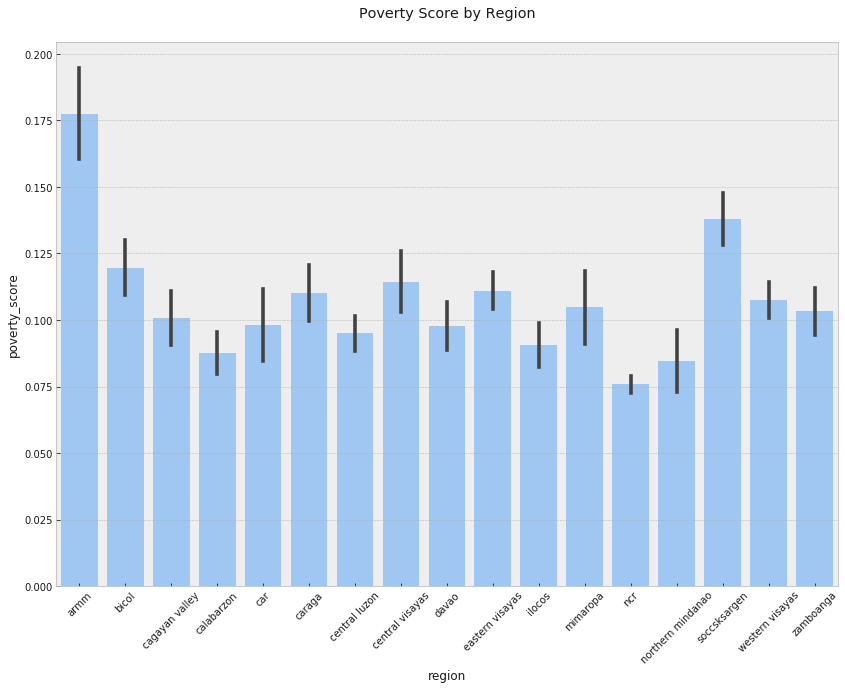
\includegraphics[width = 0.7 \textwidth]{poverty_score_region}
\end{figure}

Our predictions about the poverty in the ARMM region are consistent with our initial observations about the poverty and unemployment levels in that region.

With the predictions of poverty grouped by gender and region in the FIES dataset, we can do a merge where we will join every mean grouped poverty score to every Kiva loan record by region and gender. We can now investigate the relationship between the granted loan amount and the corresponding poverty score for each region. This could help us identify areas where Kiva can invest more and have additional positive impact.

\begin{figure}[H]
\caption{Mean Poverty Score and Mean Loan Amount by Region}
\centering
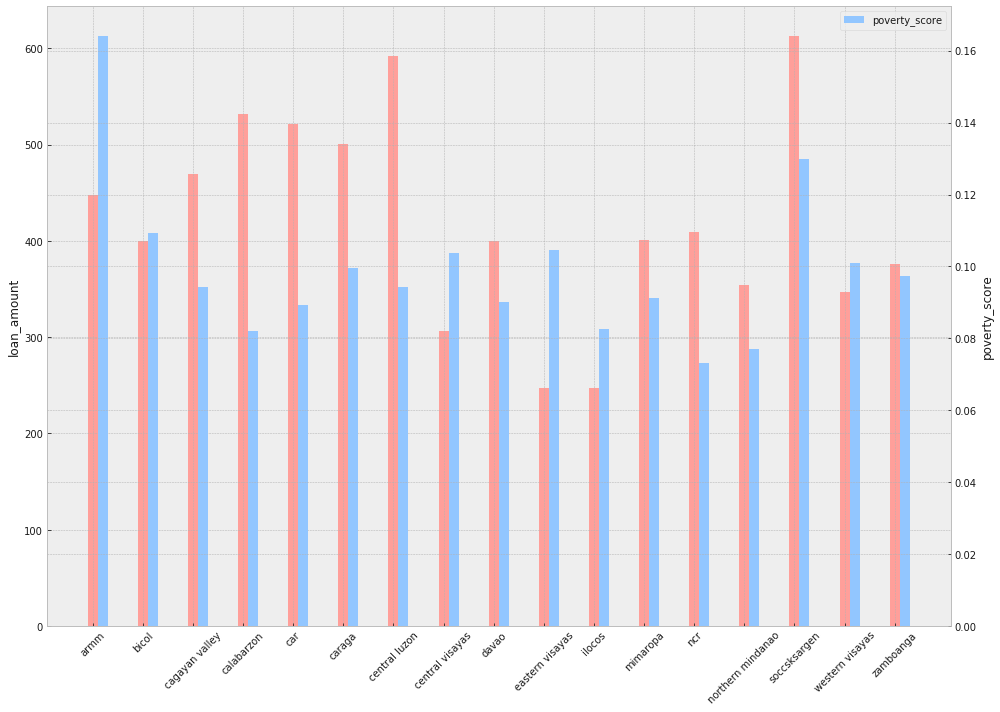
\includegraphics[width = 0.7 \textwidth]{poverty_score_loan_region}
\end{figure}

The Kiva organization could increase its footprint in the ARMM and Eastern Visayas regions and thus contribute greatly to their improvement.

\subsection{Reflection}
%In this section, you will summarize the entire end-to-end problem solution and discuss one or two particular aspects of the project you found interesting or difficult. You are expected to reflect on the project as a whole to show that you have a firm understanding of the entire process employed in your work. Questions to ask yourself when writing this section:
%Have you thoroughly summarized the entire process you used for this project?
%Were there any interesting aspects of the project?
%Were there any difficult aspects of the project?
%Does the final model and solution fit your expectations for the problem, and should it be used in a general setting to solve these types of problems?

The main reason for Kiva to create the poverty scoring challenge is to be able to better target underprivileged individuals. That’s why in this project, we decided to act as practically as possible and focus on the most important region for Kiva’s lending operation - the Philippines. Our challenge then was to define poverty and to find some data to help us derive it. For our poverty definition, we selected ‘the lack of income’ or the inverse of the income’s normalized values for the country.

We were then faced with another challenge - to find data that contains both income and predictors of income. That data also had to cover all the regions of interest (the regions in the Philippines). We chose the Philippine Family Income and Expenditure Survey produced by the Philippine Statistical Authority.

The next step in our work was to transform the FIES data to a state usable by machine learning algorithms. That is, all numeric columns and one hot encoded categorical variables. We spent a large chunk of the project effort mapping, refining and transforming the FIES data set.

One of the serious challenges of the project was to map the loan location from the Kiva loans data set to regions in the Philippines using our naming convention. The reason for that was that the ‘region’ field in the Kiva loans dataset actually contains free-form location description. In the easiest (and most prolific) case, the location description consisted of province name and city name separated by comma. In other cases, the description contained only a city name. Yet in other cases, the settlement name was that of a minor population center that we couldn’t match to any major cities or provinces. Thus we ended with 150 000 successfully matched regions. Having the regions and genders allowed us to match the eventual poverty score derived from the FIES data set and join it to the Kiva loans data set.

The next task on our list was the development of the model itself. To that end we began by exploring the correlation between the income and other variables in the transformed FIES data set. We removed some other forms of income that had values close to our target variable. We then saw that several features from the FIES data set seemed to correlate highly with our income target. Those were: the food expenses, the farming expenses, the number of communication devices and the existence of some home appliances (refrigerator, AC, etc.).

We then normalized the data and passed it through several models and compared their performance to three dummy regressors. Our initial model choices were: AdaBoost regressor, Support Vector Machines regressor, Stochastic Gradient Descent regressor, Decision Tree regressor, Linear regression and Multi Level Perceptron regressor. Our dummy regressors were objects that predicted only (0, 0.5 and 1) respectively. We then recorded the results of all models on our selected evaluation metrics. Those metrics were: mean squared error, R2 score, mean squared log error and explained variance score.

We selected the 4 best performing models and made sure that their performance was better than that of the dummy regressors. We then derived the most important features for each of the models. We inspected the features and selected one model with its two top-performing features. Those were, respectively, the Decision Tree regressor with its food expenses and farming expenses features. Both features combined added to more than 90\% of the feature weight. This allowed us to construct a lean, well explainable model that could be implemented in the field (e.g. by adding 2 simple questions to the loan application form).

We then derived the poverty metric out of the predicted income for all rows in the transformed FIES data set. We grouped the predictions for the entire dataset by region and gender and joined them to the Kiva loans data set. Thus we had a poverty metric for every loan record. In the end, we performed some visualizations of the results and investigated the poverty levels by region, gender, and compared them to the average granted loan amount per region.

\subsection{Improvement}
%In this section, you will need to provide discussion as to how one aspect of the implementation you designed could be improved. As an example, consider ways your implementation can be made more general, and what would need to be modified. You do not need to make this improvement, but the potential solutions resulting from these changes are considered and compared/contrasted to your current solution. Questions to ask yourself when writing this section:
%Are there further improvements that could be made on the algorithms or techniques you used in this project?
%Were there algorithms or techniques you researched that you did not know how to implement, but would consider using if you knew how?
%If you used your final solution as the new benchmark, do you think an even better solution exists?

The Kiva organization needs a truly global model in order to be able to successfully assist underprivileged individuals around the World. Unfortunately, our current work only covers the Philippines. Even though that is the country, where Kiva grants most of its loans, the model could be much more global. To achieve that we will need to gather other household surveys and income data from other countries.

We can then transform them and find standard features available in all countries. We can then unite all the datasets and normalize the resultant data set again. This will give us a global measure of income and therefore - poverty.

Such a global solution will produce even better results for the poverty score since the normalized predicted income will be scaled across the world. This means that countries with populations having consistently low income will appear as poor compared to other, more economically-developed ones. This will give Kiva the opportunity to target poverty on any geographical scale: continent, country, region, province, etc. Of course this would entail currency conversion, standardization and many other challenges. However, a global poverty metric could dramatically improve Kiva’s positive impact on the World.

%Before submitting, ask yourself. . .
%Does the project report you’ve written follow a well-organized structure similar to that of the project template?
%Is each section (particularly Analysis and Methodology) written in a clear, concise and specific fashion? Are there any ambiguous terms or phrases that need clarification?
%Would the intended audience of your project be able to understand your analysis, methods, and results?
%Have you properly proof-read your project report to assure there are minimal grammatical and spelling mistakes?
%Are all the resources used for this project correctly cited and referenced?
%Is the code that implements your solution easily readable and properly commented?
%Does the code execute without error and produce results similar to those reported?
\end{document}
